\subsection{August 14, 2008}
\subsubsection*{The Background}
Despite yesterday's fairly positive reading, I'm still operating in that
pessimistic sort of vein.  While less focused on relationships, the
question of money is still bothering me quite a bit, and that's leading
to me being rather down on myself about other things.

In particular, I'm rather concerned about my ability to focus on one
thing for any extended period of time.  The most obvious object of this
focus is this project itself.  I worry that I can't complete even 78
readings for myself and others.  This is a perennial problem for me, and
I often find myself flitting between interests, whether or not I have
completed any projects begun in the previous interestes.  For example,
recently, I've gone through cooking, brewing, my own small business,
programming, guns, and so on.

What's concerning me is that I worked on the problem of being stuck, and
I'm afraid that, once I start moving again, I'll fall into old habits and
start moving in too many directions at once.

\subsubsection*{The Drawing}
Still feeling in a much brighter mood than the previous day, I chose the
\textbf{Universal Waite}\cite{tarotRWS} deck - a recoloring of the RWS deck using colored
pencils to soften all of the harsh colors in the original block-printed
cards.  Additionally, I drew a card earlier in the day just to think on
and try to focus my thoughts and get in the mood for the day - I drew
the Eight of Swords.

The reading was done in a modified version of Rachel Pollack's Work Cycle
spread\cite{pollack97}.  Since I was working from her book, which
features the RWS deck heavily, the spread felt particularly fitting, and
I even deigned to introduce the element of reversed cards.  I normally
work with elemental dispositions for the rather embarassing reason of
the fact that having the cards facing different ways grates on my
nerves.  The spread was modified to leave off the `inner and outer
being' cards because I was running a little short on time.

From left to right, the cards were:
\begin{itemize}
  \item Past Experience: The Star reversed
  \item Expectations: Nine of Wands reversed
  \item Work: Knight of Swords reversed
  \item Work: Nine of Pentacles
  \item Work: Page of Pentacles reversed
  \item Outcome: Five of Wands revesred
  \item Result: Eight of Pentacles reversed
\end{itemize}
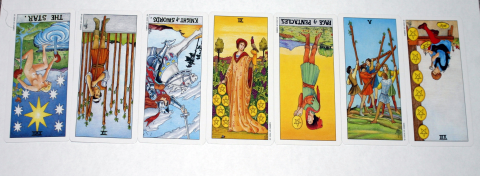
\includegraphics{image8-14-08.png}

\subsection*{The Reading}
The eight of swords shows a man with eight swords stuck in his back and
ear as he lies on the beach.  There is no blood coming from his body.
This image describes the ultimate in over reaction.  Where one sword
would've sufficed, eight have been used.  The lack of blood shows
surreality, as in the man may not actually be a man at all, as if eight
swords have been driven through a ghost, hallucination, or shadow of an
idea on this beach, right at the shore where the conscious meets the
subconscious.  I think that this card, as my `card of the day' of sorts,
is telling me to relax.  I have spent this time working with my
stressors --- getting away from some, integrating others --- and now I'm
creating more for myself by overreacting at imaginary things from the
depths of my subconscious.  With this in mind, I drew my reading for the
day, immediately surprised by only one upright card.

The Star, following immediately after The Tower, suggests a time of
healing.  Not only is the unconscious exposed and beginning to blend
with the conscious mind, but unlike The Tower, which describes the same
idea, The Star deals more with the calm after the storm --- the period
spent healing that rent caused by the fall from The Tower.  Reversed, we
are cut off from that calm, and that fear from our fall turns to
insecurity or even arrogance.  As it takes its place in my past
experience, I see that as an incomplete use of my flitting interests:
those things that distract me from stressors in order to help me heal
are not being carried out to completion, and instead of healing over,
I'm left with scars.  This echoes my desire to follow through with this
project to completion.  This, of all of my projects, is overt
self-therapy, as it's no secret that I am using this, in part, to help
get over a real ``Tower'' of a summer.

This moves into my expectations for this Work: the Nine of Wands shows a
man ready and wary, keeping his eyes out from enemies, ones that may or
may not still be enemies.  The card tells of wariness and strenght, but
also of seeing fights where there may in fact be none at all.  Reversed
twists that meaning to seeking a way out of this constant cycle, either
from being overwhelmed by the aversions or simply distressed by them.
While this is all well and good, it should be noted that sometimes these
defenses are built up for a reason, and should not be dropped lightly.
There are cases where such defenses are necessary, and I think I'm
focusing too much on these right now.  I think that opening myself up
through the cards is one case where I will \emph{have} to drop those
defenses and seek another way; I consciously know this, and expect
that this experiment will help.

The three cards of the Work group show what Pollack describes as
``\ldots{}situ-ations, influences, or attitudes that the person can use
or must overcome.''  In my case, more warnings are present.  The Knight
of Swords reversed suggests wildly casting about, showing a need to make
careful decisions and to be aware of my situation.  The Nine of
Pentacles is a card of success due to sacrifice; I need to be mindful
that this sacrifice really is for the better and not let the fact that I
am sacrificing something get in the way --- the reward is always greater
for the sacrifice.  Finally, the Page of Pentacles reversed warns again:
without a sense of hard work, all of the focus and grounded-ness of the
pentacles is liable to dissipate, leading to what Waite called
`prodigality'.

Taken together as a group these cards paint a picture of what needs to
be done.  While I know that I am working towards avoiding this casting
about ceaselessly for something with which to help myself, I will need
the Pentacles' focus and the sacrifice showin in the Nine.  To me, I see
this as sacrificing time and energy, both of which seem to be
increasingly parcelled out in today's world.  Free time is always seen
as valuable, and it's difficult to give some of mine up to a task that
requires such mental exertion and, honestly, leaves me intellectually
winded for a period afterwards.  I needn't be afraid of this sacrifice,
however, as expensing that energy will help me in at least two ways: not 
only with the therapy inherent in this project; but also as a sort of
exercise, building up my intellectual stamina, as it were, getting my
mind used to working in these intricate patterns.
%KnS R - wild casting about, requires careful decisions and awareness
%9P - success with sacrifice, if sacrifice seems too great, reconsider
%the value of the rewards we'll gain - always great
%PP R - without sense of hard work, dissipates; prodigality

Following the Work group of cards is the final combination of Outcome
and Result.  While Outcome stands for the likely way that things will
develop, Result implies a more personal side, showing how the outcome
with affect the subject or their reaction to it.  For my reading, these
cards came out fairly disheartening at first.  The Five of Wands
reversed suggests rules abandoned in this intellectual battle of mine, leading to
nastier combat.  I'll clearly have to do more to stick with this
interest, lest it fall by the wayside - perhaps things out of the
ordinary for me.  The Eight of Pentacles reversed on the other hand,
shows frustration and lack of fulfillment due to looking strictly for
success rather than working for the sake of work.  This meaning grated
on my nerves until I saw it as just another step in the path: not only
is success in the standard sense of strict completion unlikely, but I 
am almost certain to become frustrated by not really having an ending
point to this at all.  After all, this is only seventy-eight tarot
readings, which is only a little more than a fifth of a year if they are
done one a day!  I could change so much more, reading every day for the
rest of my life, and still never reach an end to this experiment, as
there is always more change to be had.  This is certainly something I
must learn to accept if I am to keep this project and others going
strong.
% 5W R - rules abandoned, battle is nastier, have to do more to
% stickwith interest?
% 8P R - frustration/unfulfilled from looking for Success, not work ?
